\chapter{Introduction}
	Computer vision is the development of models and algorithms, to interpret digital images and to get a better understanding of the visual world. One aspect of understanding the world is the recovery of shapes. The goal of shape recovery is to obtain three dimensional informations about a scene or an object from one or more 2D images. The estimated shape can be represented in various ways. 
	\\
	One way to represent the shape of an object is using depth $Z(x,y)$. Therefor either the relative surface height above the x-y plane ore the relative distance from surface to camera is measured. The depth map encode near points on the surface darker and distant point lighter to a gray scale image. 
	\\
	Another way to express the shape of an object is to use surface normal $(n_x, n_y, n_z)$. The surface normal is the direction of a vector perpendicular to the tangent plane of the surface point and can be calculated by taking the cross product $l \times s$ of two vectors that span the plane, e.g. between the vector of incident ray $l$ and the orientation vector of the camera $s$. To obtain depth informations, the surface gradient $(p,g) = (\frac{\partial z}{\partial x}, \frac{\partial z}{\partial y}) $ is used, since it indicates the rate of the depth change along the $x$- and $y$-axis. For visualization the normal map then encode the direction of the vectors to the RGB colors.
	%TODO Figure normal map (koordinaten system) depth bsp 
	\\ 
	\\
	Shape recovery is a classic and hard to solve problem in computer vision. Therefore several methods and techniques have been developed~\cite{Horn_SHAPE_FROM_SHADING_1970, Shape_from_X_psychophysics_and_computation}. In computer vision techniques to recover the shape of an object are called shape-from-X, where X can stand for: focus, motion, shading, stereo, texture, etc. In this thesis the shape-from-shading technique will be used to recover an objects shape. Shape-from-shading uses the shading of an object's surface to recover informations about the 3D shape of this object. Artists early learned the principle of using lighting and shading to create the illusion of depth in there paintings. To solve shape-from-shading it is important to a
	%TODO beschreiben warum shape from shading schwer ist
	\\
	\\
	%TODO Problem Bild verarbeitung vortschritt in neuronalen Netzen usw.
	Humans solve problems like shape recovery (shape-from-shading) with ease. However they are very hard to solve for a computer.	
	\\ 
	\\	
	MarrNet~\cite{MarrNet} is an two step end to end trainable model that uses an encoder-decoder convolutional neuronal network architecture in addition to reconstruct the three-dimensional shape of an object using 2.5D sketches. Therefor the first step of the Model predicts the depth map, surface normals and silhouette of an object given a single RGB image. However like the most shape-from-shading techniques MarrNet assume orthographic images, which are not very realistic. 
	\\
	The hypotheses of this theses is that with increasing perspective distortion the accuracy decreases. Therefore a large scale dataset (chapter \ref{sec:dataset}), containing four types of image projections, were created, trained and evaluated (chapter \ref{sec:exp}) on the MarrNet model.
	% \begin{figure}
	%	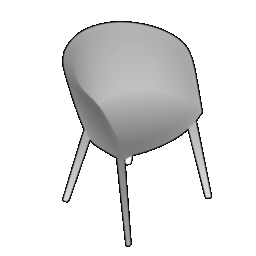
\includegraphics[height=0.1\textheight]{introduction_depth.png}
	%	\caption{A boat.}
	%	\label{fig:boat1}
	% \end{figure}
